\documentclass[14pt,aspectratio=169]{beamer}
\setbeamertemplate{caption}[numbered]
\setbeamertemplate{caption label separator}{:}
\setbeamercolor{caption name}{fg=normal text.fg}
\usepackage{amssymb,amsmath}
\usepackage{ifxetex,ifluatex}
\usepackage{fixltx2e} % provides \textsubscript
\usepackage{lmodern}
\ifxetex
  \usepackage{fontspec,xltxtra,xunicode}
  \defaultfontfeatures{Mapping=tex-text,Scale=MatchLowercase}
  \newcommand{\euro}{€}
\else
  \ifluatex
    \usepackage{fontspec}
    \defaultfontfeatures{Mapping=tex-text,Scale=MatchLowercase}
    \newcommand{\euro}{€}
  \else
    \usepackage[T1]{fontenc}
    \usepackage[utf8]{inputenc}
      \fi
\fi
% use upquote if available, for straight quotes in verbatim environments
\IfFileExists{upquote.sty}{\usepackage{upquote}}{}
% use microtype if available
\IfFileExists{microtype.sty}{\usepackage{microtype}}{}
\PassOptionsToPackage{hyphens}{url}
\usepackage{hyperref}

% Comment these out if you don't want a slide with just the
% part/section/subsection/subsubsection title:
\AtBeginPart{
  \let\insertpartnumber\relax
  \let\partname\relax
  \frame{\partpage}
}
\AtBeginSection{
  \let\insertsectionnumber\relax
  \let\sectionname\relax
  \begin{frame}[plain]
    \tableofcontents[currentsection]
  \end{frame}
}
\AtBeginSubsection{
  \let\insertsubsectionnumber\relax
  \let\subsectionname\relax
  \frame{\subsectionpage}
}

\setlength{\parindent}{0pt}
\setlength{\parskip}{6pt plus 2pt minus 1pt}
\setlength{\emergencystretch}{3em}  % prevent overfull lines
\setcounter{secnumdepth}{0}
% Thanks Richard Darst on how to get a nice Beamer theme.
% See http://rkd.zgib.net/wiki/DebianBeamerThemes

\usepackage{multicol}
\usepackage{tikz}
\usetikzlibrary{positioning}
\usepackage{ctable}

\usebackgroundtemplate{
\includegraphics[width=\paperwidth]{images/swirl-lightest.pdf}}
\logo{
\includegraphics[viewport=274 335 360 440,width=1cm]{images/openlogo-nd.pdf}}

\definecolor{debianred}{rgb}{.780,.000,.211} % 199,0,54
\definecolor{debianblue}{rgb}{0,.208,.780} % 0,53,199
\definecolor{debianlightbackgroundblue}{rgb}{.941,.941,.957} % 240,240,244
\definecolor{debianbackgroundblue}{rgb}{.776,.784,.878} % 198,200,224

\usetheme{Boadilla}
\setbeamertemplate{navigation symbols}{}

\usecolortheme[named=debianbackgroundblue]{structure}
\setbeamercolor{normal text}{fg=black}
\setbeamercolor{titlelike}{fg=debianblue}
\setbeamercolor{sidebar}{fg=debianred,bg=debianbackgroundblue}

\setbeamercolor{palette sidebar primary}{fg=debianred}
\setbeamercolor{palette sidebar secondary}{fg=debianred}
\setbeamercolor{palette sidebar tertiary}{fg=debianred}
\setbeamercolor{palette sidebar quaternary}{fg=debianred}

\setbeamercolor{section in toc}{fg=debianred}
\setbeamercolor{subsection in toc}{parent=debianred}

\setbeamercolor{item}{fg=debianred}

\setbeamercolor{block title}{fg=debianblue}

\title[Reproducible Builds]{Construcciones reproducibles en Debian\\
(Debian Reproducible Builds)}
\subtitle{Un camino verificable desde el origen hasta el binario}
\author[Jathan]{%
   \texorpdfstring{
            Jonathan Bustillos Osornio\\
            \href{mailto:jathanblackred@openmailbox.org}{\texttt{jathanblackred@openmailbox.org}}
   }{Jathan}}
\institute[Debian]{}
\date[CubaConf Habana 2017]{%
 CubaConf Habana\\
 \small
 2017-11-08}

\begin{document}
\begin{frame}
\titlepage
\end{frame}

\begin{frame}
 \frametitle{Acerca de Jathan}

 \begin{itemize}
  \item \small{\texttt{3006 B194 2622 24C7 1607 F72B 52E4 5D29 AA34 EFC5}}
  \item Usuario de Debian desde el 2008 y contribuidor desde el 2011.
    \begin{itemize}
    \item \texttt{Equipo de localización al español (2011)}
    \item \texttt{Debian Reproducible Builds (2017)}
   \end{itemize}   
  \item Participante en algunos eventos de Debian desde el 2011.
   \begin{itemize}
    \item \texttt{Día Debian}
    \item \texttt{Fiestas de instalación}
    \item \texttt{DebConf}
   \end{itemize}
 \end{itemize}
\end{frame}

\begin{frame}
 \frametitle{Equipo Debian Reproducible Builds}
 \begin{center}
  \begin{columns}
   \scriptsize
   \column{.30\linewidth}
    {akira} \\
    {Alexis Bienvenüe} \\
    {Andrew Ayer} \\
    {Asheesh Laroia} \\
    Boyuan Yang \\
    {Ceridwen} \\
    {Chris Lamb} \\
    {Chris West} \\
    {Christoph Berg} \\
    Clint Adams \\
    Dafydd Harries \\
    {Daniel Kahn Gillmor} \\
    {Daniel Shahaf} \\
    Daniel Stender \\
    David Suarez \\
    {Dhole} \\
    Drew Fisher \\
    Emmanuel Bourg \\
    Emanuel Bronshtein \\
    \column{.30\linewidth}
    Esa Peuha \\
    {Fabian Wolff} \\
    {Guillem Jover} \\
    Hans-Christoph Steiner \\
    Harlan Lieberman-Berg \\
    {Helmut Grohne} \\
    {Holger Levsen} \\
    HW42 \\
    Intrigeri \\
    {Jelmer Vernooij} \\
    \only<1>{Jonathan Bustillos}\only<2>{{\color{debianblue} Jonathan Bustillos}} \\
    {josch} \\
    Juan Picca \\
    Juliana Rodrigues \\
    {Lunar} \\
    Maria Glukhova \\
    Mathieu Bridon \\
    {Mattia Rizzolo} \\
    Nicolas Boulenguez \\
    {Niels Thykier} \\
   \column{.30\linewidth}
    Niko Tyni \\
    {Paul Wise} \\
    Peter De Wachter \\
    Philip Rinn \\
    {Reiner Herrmann} \\
    Robbie Harwood \\
    {Santiago Vila} \\
    {Sascha Steinbiss} \\
    {Satyam Zode} \\
    {Scarlett Clark} \\
    {Stefano Rivera} \\
    {Stéphane Glondu} \\
    {Steven Chamberlain} \\
    Tom Fitzhenry \\
    Vagrant Cascadian \\
    {Valerie Young} \\
    Valentin Lorentz \\
    {Wookey} \\
    {Ximin Luo} \\
  \end{columns}
 \end{center}
\end{frame}

\section{Introducción}

\begin{frame}
\frametitle{El problema}

\center

\begin{tikzpicture}
\draw (-2,0) node[font=\LARGE] (Origen) { Origen };
\draw (2,0) node[font=\LARGE] (Binario) { Binario };
\draw[->,very thick] (Origen) -- (Binario) node[midway] (midbuild) {};
\draw (midbuild) node [above,color=debianred,font=\small] (Construcción) {Construcción};
\visible<2>{
\draw (0,2) node[font=\LARGE,color=debianblue] (fs) { Software Libre };
% font= specification is required to work-around a bug in md->latex conversion
\draw[->,font=\normalsize] (fs) -- (Origen) node[midway,left=0.2cm,color=debianred,font=\footnotesize,align=center]{Libertad\\para estudiar};
\draw[->,font=\normalsize] (fs) -> (Binario) node[midway,right=0.2cm,color=debianred,font=\footnotesize,align=center]{Libertad\\para ejecutar};
}
\visible<3->{
\draw (-4,-1) node[font=\small,color=debianblue] (Verificado) { Puede ser verificado };
\draw (4,-1) node[font=\small,color=debianblue] (Usado) { Puede ser usado };
\path (Verificado) edge[->,bend left=30] (Origen);
\path (Usado) edge[->,bend right=30] (Binario);
}
\visible<4->{
\draw (0,-2) node[font=\LARGE,color=debianred,align=center] (Prueba) { ¿Podría obtener una prueba? };
\path (Prueba) edge[->] (midbuild);
}
\end{tikzpicture}

\end{frame}

\section{Motivación}

\begin{frame}[fragile]
 \frametitle{El problema: tenemos que creer}
 \begin{itemize}
  \item ¡El Software Libre es grandioso: ¡Puedes estudiarlo, modificarlo, compartirlo y usarlo!
  \item<2-4> Estudiamos, modificamos y compartimos el código fuente.
  \item<2-4> Usamos binarios.
  \item<3-4> Necesitamos creer que nuestros binarios provienen del código fuente del que se dice que provienen.
  \item<4> \textbf{No queremos creer.}
 
 \end{itemize}
\end{frame}


\begin{frame}
 \frametitle{El problema en mayor detalle}

 \begin{center}
  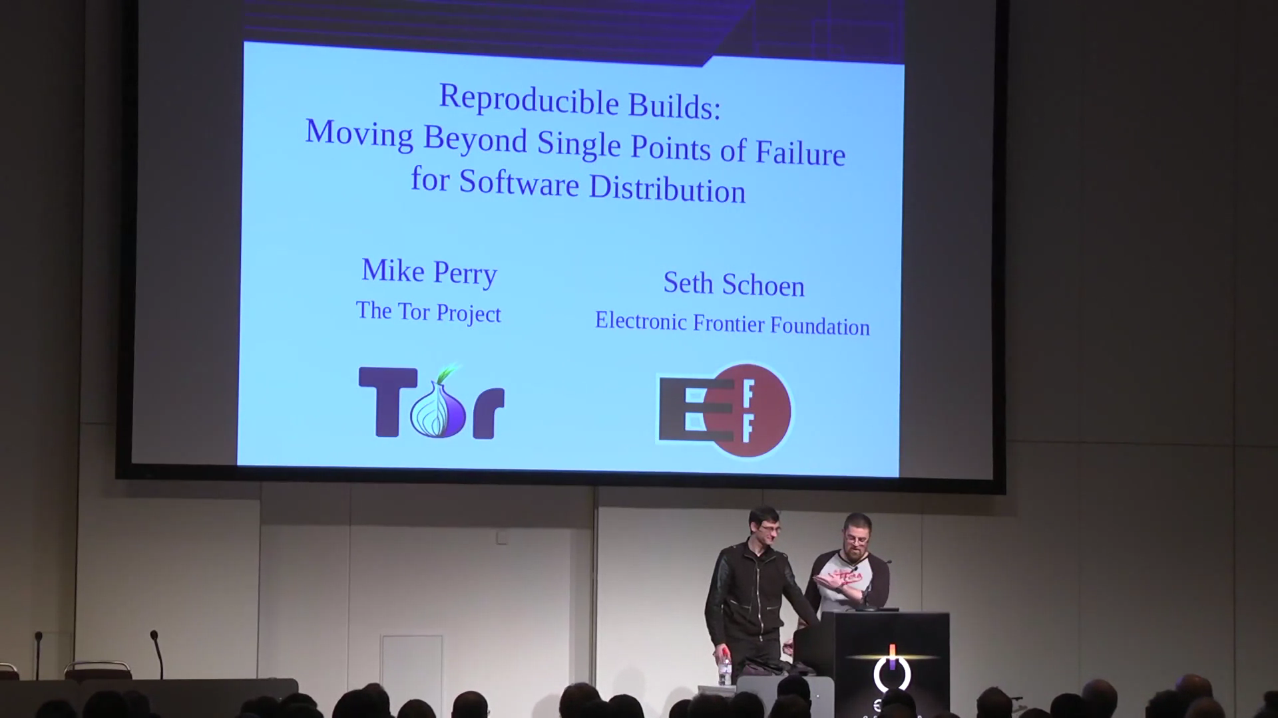
\includegraphics[width=0.7\textwidth]{images/31c3.png}

  Disponible en \url{media.ccc.de}, 31c3
 \end{center}
\end{frame}

\begin{frame}[fragile]
 \frametitle{Algunos ejemplos de esa plática 31c3}
 \begin{itemize}
  \item CVE-2002-0083: exploit de escalación a root en \texttt{sshd}, una diferencia de un sólo bit en el binario.
  \item<2-5> La plática 31c3 tiene una demostración en vivo con un módulo del kernel modificando el código fuente de un programa.
  \item<3-5> ¿Cómo puedes estar seguro qué se está ejecutando en tu máquina o en 
  un paquete como un demonio de red conectado a otras computadoras? ¿Alguna vez 
  dejas tus computadoras físicamente solas? 
  \item<4-5> ¿Cuánto le pagas a tus administradores? ¿Suficiente cómo para resistir un ataque que implique      inmensas pérdidas valiosas?
  \item<5> Desafíos legales ¿Te podrías ver obligado a desarrollar backdoors en algunos de tus
  programas para algunos clientes?
 \end{itemize}
\end{frame}

\begin{frame}[fragile]
\frametitle{Otro ejemplo de la vida real}

En una conferencia de la CIA en 2012:

\begin{center}
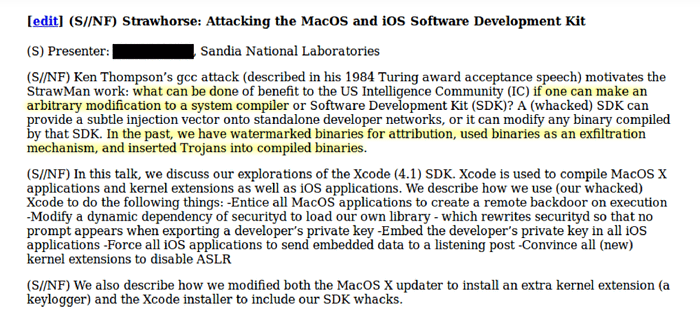
\includegraphics[width=0.8\textwidth]{images/strawhorse.png}

{\footnotesize 
\url{firstlook.org/theintercept/2015/03/10/ispy-cia-campaign-steal-apples-secrets/}
}
\end{center}

\end{frame}

\begin{frame}
\frametitle{La solución}

\begin{center}
\Large
Permitir a cualquier persona\\
reproducir paquetes binarios\\
idénticos de un origen dado.
\end{center}

\end{frame}

\begin{frame}
\frametitle{La solución}

\begin{center}
Nosotros llamamos a esto:

\huge
«Construcciones reproducibles» \\
\begin{LARGE}
(Reproducible Builds)
\end{LARGE}
\end{center}

\end{frame}

\begin{frame}
\frametitle{¡No es moda ni capricho!}

\begin{itemize}
\item Bitcoin - 2011 (\textbf{Hecho})
\item Coreboot - 2016 (\textbf{Hecho})
\item Debian - 2014 trabajo iniciado y 2017 en debian-policy (\emph{En progreso})
\item FreeBSD - 2016 (\emph{En progreso})
\item NetBSD - 2016 (\emph{En progreso})
\item OpenWrt - 2016 (\emph{En progreso})
\item Tails - 2017 (\emph{En progreso})
\item Tor - 2013 (\textbf{Hecho})
\item \ldots{}
\end{itemize}

\end{frame}

\begin{frame}[plain]
\begin{center}
\Huge Debería convertirse en la \textbf{norma}.

\visible<2>{\normalsize{ Queremos cambiar el significado de «Software Libre»:

  ¡Sólo es Software Libre si es reproducible!}}

\end{center}
\end{frame}

\begin{frame}
\frametitle{Múltiples aspectos}

\begin{itemize}
\item Sistema de construcción determinista \\
  \textit{\small Para aquellos que escriben código fuente}
\item Entorno de construcción reproducible \\
  \textit{\small Para aquellos que crean binarios para otros}
\item Distribuir el entorno de construcción \\
  \textit{\small Para aquellos que distribuyen binarios al mundo}
\item \color{gray}{Realizar una reconstrucción y verificar los resultados} \\
  \textit{\small Para cada uno de nosotros}
\end{itemize}

\end{frame}

\section{Sistema de construcción determinista}

\begin{frame}
\frametitle{Sistema de construcción determinista}

En una palabra:

\begin{itemize}
\item Entradas estables (Stable inputs).
\item Salidas estables (Stable ouputs).
\item Capturar lo menos posible del entorno.
\end{itemize}
\end{frame}

\begin{frame}
 \frametitle{Problemas comúnes}

 \begin{itemize}
  \item Timestamps (tiempo actual de registro)
  \item Orden del archivo
  \item Pseudo aleatoriedad:
   \begin{itemize}
    \item Rutas temporales de archivos
    \item UUID
    \item Protección contra ataques de complejidad
   \end{itemize}
  \item Relación a CPU y memoria:
   \begin{itemize}
    \item Optimizaciones de código para la clase actual de CPU
    \item Registro de direcciones de memoria
   \end{itemize}
  \item Ruta de la construcción
  \item Configuración regional y zona horaria
 \end{itemize}
\end{frame}

\begin{frame}[plain]
 \begin{tikzpicture}[remember picture,overlay]
  \node[at=(current page.center)] {
    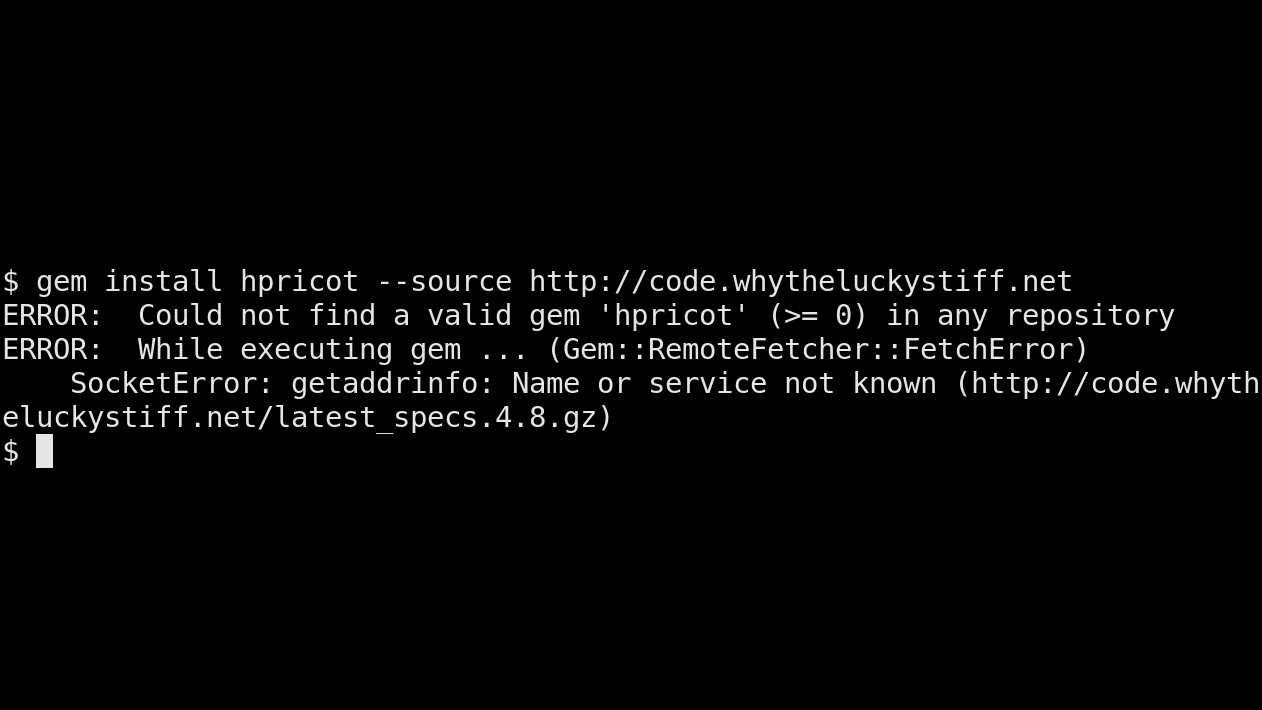
\includegraphics[width=\paperwidth]{images/why_is_gone.png}
  };
 \end{tikzpicture}
\end{frame}

\begin{frame}[fragile]
 \frametitle{Las entradas volátiles pueden desaparecer}

 \begin{itemize}
  \item No confíes en la red
  \item Si lo haces:
   \begin{itemize}
    \item Verifica contenido usando sumas de verificación
    \item Ten una copia de seguridad
   \end{itemize}
  \item El distribuidor binario debería proporcionar una alternativa
\end{itemize}

\begin{block}{\small FreeBSD lo hace bien}\footnotesize
\begin{semiverbatim}
\$ grep MASTER\_SITES Makefile
MASTER\_SITES= http://gondor.apana.org.au/~herbert/dash/files/
\$ cat distinfo
SHA256 (dash-0.5.8.tar.gz) = c6db3a237747b02d20382a761397563d813b306c020ae28ce25…
SIZE (dash-0.5.8.tar.gz) = 223028
\$ wget http://distcache.freebsd.org/ports-distfiles/distfiles/dash-0.5.8.tar.gz
\end{semiverbatim}
\end{block}
\end{frame}

\begin{frame}[plain]
 \begin{tikzpicture}[remember picture,overlay]
  \node[at=(current page.center)] {
    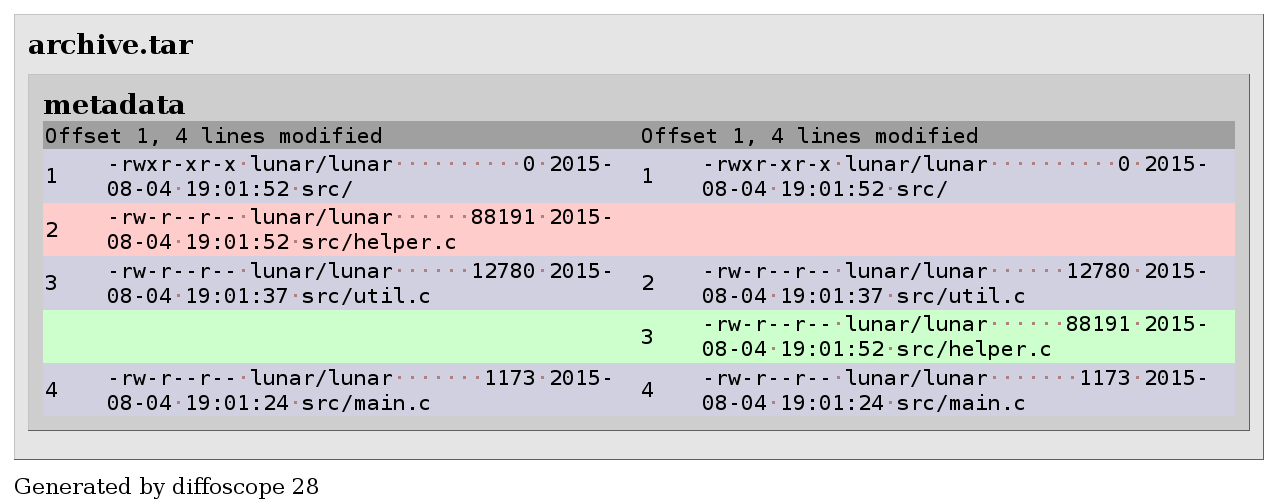
\includegraphics[width=\paperwidth]{images/filesystem_order_in_tarball.png}
  };
 \end{tikzpicture}
\end{frame}

\begin{frame}[fragile]
 \frametitle{Orden estable para las entradas}

 \begin{itemize}
  \item Siempre procesa múltiples entradas en el mismo orden
  \item ¡Las listas de directorios no son estables!
  \item<2-> Soluciones:
   \begin{itemize}
    \item Lista entradas explícitamente
    \item<3-> Usa clasificación
    \item<4> \alert{Pero ten cuidado con la diferencia entre la localización y el idioma.}
   \end{itemize}
 \end{itemize}

 \begin{example}
  \begin{overprint}
   \onslide<1>
\begin{semiverbatim}
tar -cf archive.tar src
\end{semiverbatim}
   \onslide<2>
\begin{semiverbatim}
tar -cf archive.tar \\
  src/util.c src/helper.c src/main.c
\end{semiverbatim}
   \onslide<3->
\begin{semiverbatim}
find src -print0 | \only<4>{\alert{LC\_ALL=C} }sort -z |
  tar --null -T - --no-recursion -cf archive.tar
\end{semiverbatim}
  \end{overprint}
 \end{example}
\end{frame}

\begin{frame}[plain]
 \begin{tikzpicture}[remember picture,overlay]
  \node[at=(current page.center)] {
    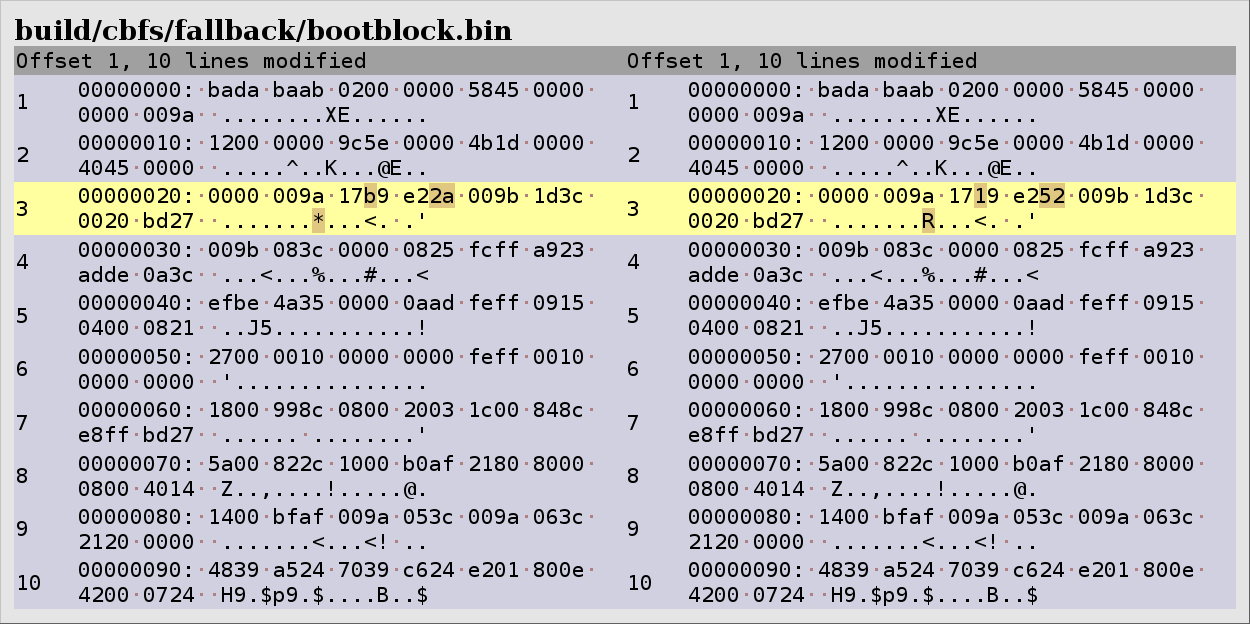
\includegraphics[width=\paperwidth]{images/uninitialized_memory.png}
  };
 \end{tikzpicture}
\end{frame}

\begin{frame}[fragile]
 \frametitle{Inicialización de un valor controlado}

 \begin{itemize}
  \item No registres memoria por accidente
  \item<2>Siempre inicializa un valor conocido
 \end{itemize}

 \begin{example}
\begin{semiverbatim}\small
static int write_binary(FILE *out, FILE *in, struct bimg_header *hdr)
\{
       static uint8_t file_buf[MAX_RECORD_BYTES];
       struct bimg_data_header data_hdr\only<2>{\alert{ = \{ 0 \}}};
       size_t n_written;

       data_hdr.dest_addr = hdr->entry_addr;
       …
\end{semiverbatim}
 \end{example}
\end{frame}

\begin{frame}[plain]
 \begin{tikzpicture}[remember picture,overlay]
  \node[at=(current page.center)] {
    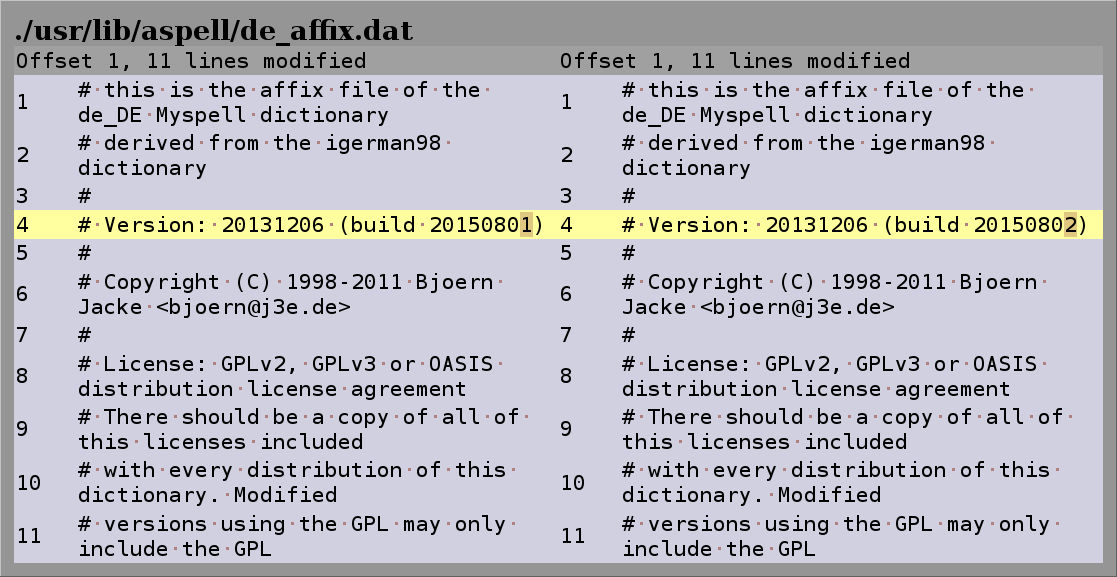
\includegraphics[width=\paperwidth]{images/varying_version.png}
  };
 \end{tikzpicture}
\end{frame}

\begin{frame}[fragile]
 \frametitle{Utiliza información de una versión determinista}

 \begin{itemize}
  \item No generes un número de versión en cada construcción
  \item<2> En su lugar, extrae información del origen:
    \begin{itemize}
      \item Revisión del sistema de control de versiones
      \item Hash del código fuente
      \item Entrada de registro de cambios
    \end{itemize}
 \end{itemize}

 \begin{example}<2>\small
\begin{semiverbatim}
\alert{VERSION=$(shell dpkg-parsechangelog | sed -n 's/^Version: *//p')}

SCONSOPTS = $(SCONSFLAGS) \alert{VERSION=$(VERSION)} \\
  PREFIX=$(PREFIX) PREFIX_CONF=$(SYSCONF) CHMDOCS=0 \\
  STRIP_CP=no \\
  $(if $(findstring nostripfull,$(DEB_BUILD_OPTIONS)),STRIP_W32=no,)
\end{semiverbatim}
 \end{example}
\end{frame}

\begin{frame}[plain]
 \begin{tikzpicture}[remember picture,overlay]
  \node[at=(current page.center)] {
    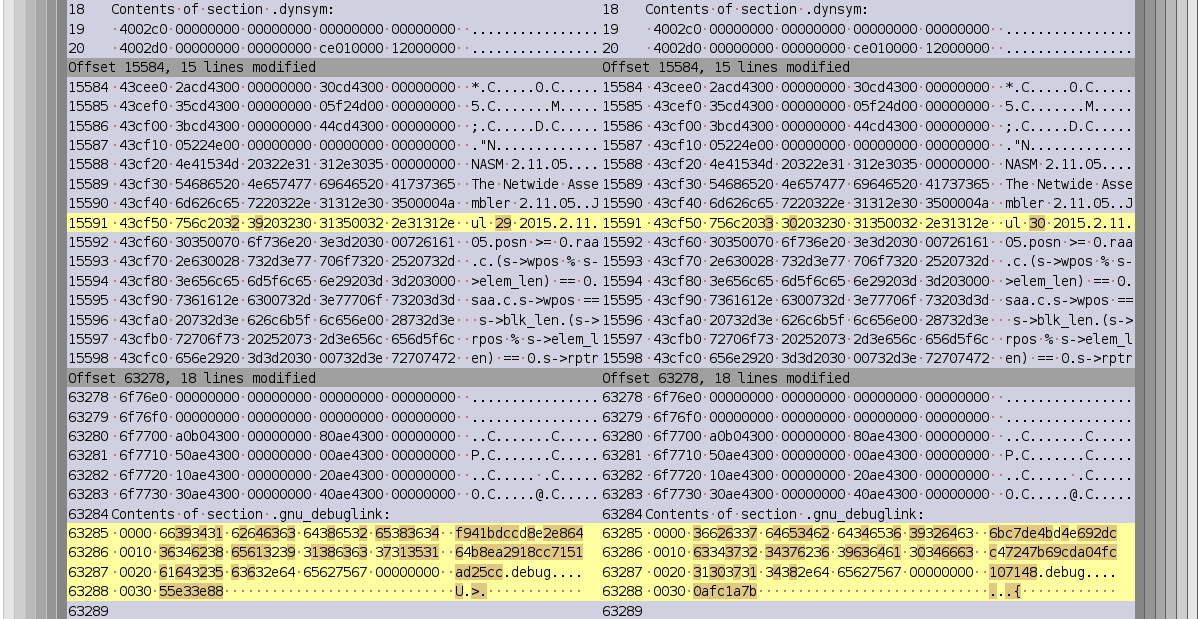
\includegraphics[width=\paperwidth]{images/timestamp_in_nasm.png}
  };
 \end{tikzpicture}
\end{frame}

\begin{frame}
 \frametitle{No registres la fecha y la hora actual}

 \begin{itemize}
  \item Evita sellos de tiempo (timestamps)
  \item<2-> Si necesitas uno:
    \begin{itemize}
      \item Utiliza la fecha del último commit en el VCS
      \item Extráelo del registro de cambios
      \item<3-> \alert{No olvides la zona horaria}
    \end{itemize}
  \item<4-> \texttt{faketime} es una opción pero tiene serios inconvenientes \\
    {\small \url{https://bugs.torproject.org/12240}}
  \item<5> Implementa \texttt{SOURCE\_DATE\_EPOCH}
 \end{itemize}
\end{frame}

\begin{frame}
 \frametitle{\texttt{SOURCE\_DATE\_EPOCH}}

 \begin{itemize}
   \item Qué es?
     \begin{itemize}
       \item Variable de entorno con un tiempo de referencia
       \item Número de segundos desde la «Época» (1970-01-01 00:00:00 +0000 UTC)
       \item Si está configurada, reemplaza "hora actual del día" (Current time of day)
       \item Implementado por \texttt{help2man}, Epydoc, Doxygen, Ghostscript (en Debian)
       \item Ha sido adoptado por otras distribuciones (openSUSE, OpenWrt,
LEDE, NetBSD, FreeBSD, Arch Linux, coreboot, Guix,. . . ) y
muchos upstreams (GCC, dpkg, rpm, mkisofs, ghostscript, libxslt,
sphinx, texlive-bin,. . . )
       \item Parches listos para GCC, \texttt{txt2man}, \texttt{libxslt}, Gettext…
     \end{itemize}
   \item<2-> Configura \texttt{SOURCE\_DATE\_EPOCH} en tu sistema de construcción
   \item<3> Agrega soporte en cualquier herramienta que escriba sellos de tiempo
 \end{itemize}

 \begin{center}
   {\small \url{https://wiki.debian.org/ReproducibleBuilds/TimestampsProposal}}
 \end{center}
\end{frame}

\begin{frame}[plain]
 \begin{tikzpicture}[remember picture,overlay]
  \node[at=(current page.center)] {
    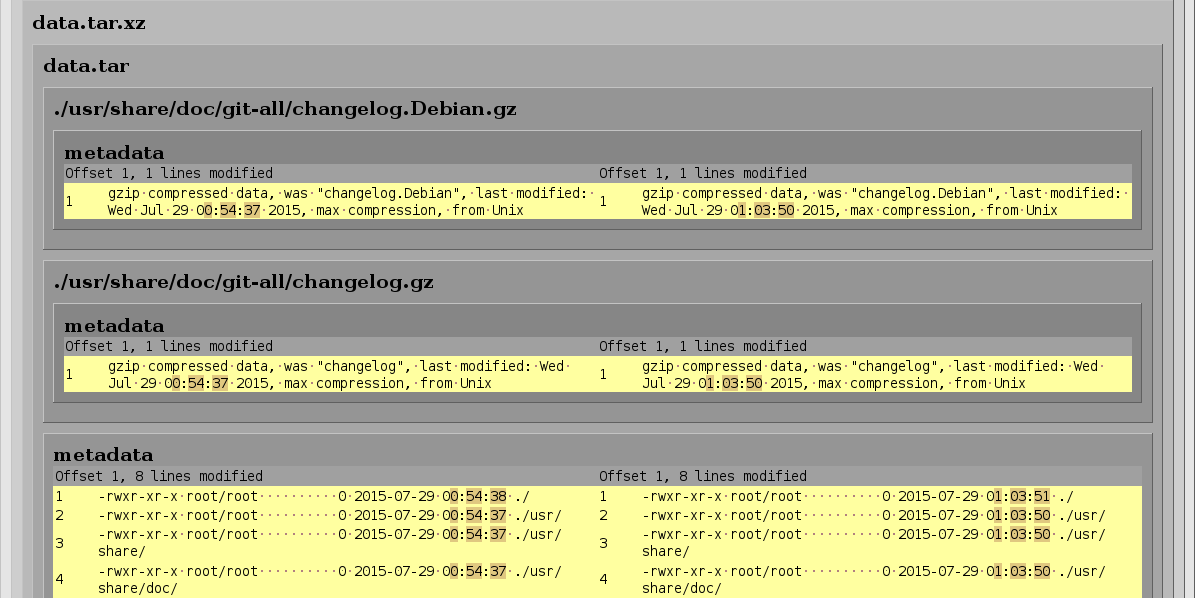
\includegraphics[width=\paperwidth]{images/timestamp_in_git_deb.png}
  };
 \end{tikzpicture}
\end{frame}

\begin{frame}[fragile]
 \frametitle{No registres la hora actual (de verdad)}

 \begin{itemize}
  \item Los archivos mantienen los tiempos de modificación en los metadatos
  \item Almacenar un archivo puede registrar el tiempo de construcción
  \item<2-> Soluciones:
   \begin{itemize}
    \item Almacenar un valor arbitrario
    \item<3-> Tiempo de modificación del archivo de preproceso
    \item<4> Archivo post-proceso
   \end{itemize}
 \end{itemize}

 \begin{example}
\begin{semiverbatim}
\only<1-3>{\visible<3>{\alert{touch --date="2015-08-13 00:00Z" build/*}}
tar\only<2>{\alert{ --mtime='2015-08-13 00:00Z'}} -cf product.tar build
}\only<4>{\textit{\color[rgb]{.7,.7,.7}# zip has no equivalent of --mtime}
zip product.zip build
\alert{strip-nondeterminism product.zip}}
\end{semiverbatim}
 \end{example}
\end{frame}

\begin{frame}[plain]
 \begin{tikzpicture}[remember picture,overlay]
  \node[at=(current page.center)] {
    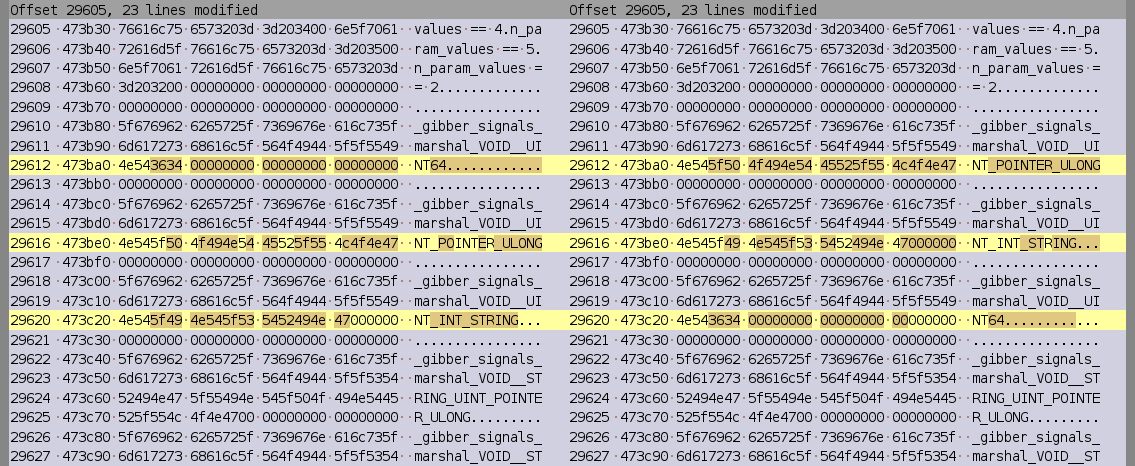
\includegraphics[width=\paperwidth]{images/random_function_order.png}
  };
 \end{tikzpicture}
\end{frame}

\begin{frame}[fragile]
 \frametitle{Orden estable para salidas}

 \begin{itemize}
  \item Siempre listas de salida en el mismo orden
  \item Problema típico: orden de las teclas con tablas hash\\
    {\small \url{perldoc.perl.org/perlsec.html#Algorithmic-Complexity-Attacks}}
  \item<2> ¡Ordenar!
 \end{itemize}

 \begin{example}
\begin{semiverbatim}
for module in \only<2>{\alert{sorted(}}dependencies.keys()\only<2>{\alert{)}}:
    version = dependencies[module]
    print('\%s (>= \%s)' \% (module, version))
\end{semiverbatim}
 \end{example}
\end{frame}

{
\usebackgroundtemplate{%
 \begin{tikzpicture}[remember picture,overlay]%
  \node[shift={(-0.2\paperwidth, -0.2\paperheight)},at=(current page.north east)] (image) {
    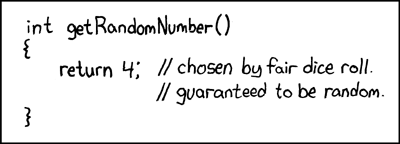
\includegraphics[width=0.3\paperwidth]{images/random_number.png}
  };
  \node[below=-0.03\paperheight of image,align=center,font=\tiny,color=gray]{XKCD \#221};
 \end{tikzpicture}%
}
\begin{frame}[fragile]
 \frametitle{Evita la aleatoriedad}

 \begin{itemize}
  \item La aleatoriedad no es determinista
  \item<2-> Siembra tu PRNG de un valor conocido
   \begin{itemize}
     \item Usa un valor fijo
     \item<3> Extrae del código fuente (nombre del archivo, contenido hash)
   \end{itemize}
 \end{itemize}

 \begin{example}
\begin{semiverbatim}\small
\$ gcc -flto -c\only<2->{ \alert{-frandom-seed=}}\only<2>{\alert{0}}\only<3>{\alert{utils.o}} utils.c
\$ nm -a utils.o | grep inline
\only<1>{0000000000000000 n .gnu.lto\_.inline.381a277a0b6d2a35}\only<2>{0000000000000000 n .gnu.lto\_.inline.0}\only<3>{0000000000000000 n .gnu.lto\_.inline.a108e942}
\end{semiverbatim}
 \end{example}
\end{frame}
}

\begin{frame}
 \frametitle{Define una variable de entorno que afecte a los resultados}

 \begin{itemize}
  \item Algunas variables de entorno afectarán a las salidas del software. Ejemplos:
   \begin{itemize}
    \item \texttt{LC\_CTIME} para las cadenas de tiempo
    \item \texttt{LC\_CTYPE} para la codificación de texto
    \item \texttt{TZ} para los tiempos
   \end{itemize}
  \item<2-> Establécelos en un valor controlado
  \item<3> \textit{No fuerces el lenguaje}
 \end{itemize}
\end{frame}

\begin{frame}
 \frametitle{Deja de registrar la información del sistema de construcción}

 \begin{itemize}
  \item No registres la información sobre el sistema de construcción, como:
   \begin{itemize}
    \item fecha y hora de la construcción
    \item nombre de equipo (hostname)
    \item ruta
    \item configuración de la red
    \item CPU
    \item variables de entorno
    \item …
   \end{itemize}
  \item<2> Si realmente quieres registrarla, hazlo fuera de los binarios
 \end{itemize}
\end{frame}

\section{Entorno de construcción reproducible}

\begin{frame}
 \frametitle{¿Qué hay en un entorno de construcción?}

 \begin{itemize}
  \item Al menos herramientas de construcción y sus versiones específicas
  \item<2> Depende de ti, dependiendo del sistema de construcción:
   \begin{itemize}
    \item arquitectura de la construcción
    \item sistema operativo
    \item \textit{ruta de la construcción}
    \item \textit{fecha y hora de la construcción}
    \item …
   \end{itemize}
 \end{itemize}
\end{frame}

\begin{frame}
 \frametitle{Construye desde el origen}

 \begin{itemize}
  \item Herramientas de construcción que afectan la salida del origen
  \item Registrar la versión / tag / git commit
  \item Enfoque usado por Coreboot, OpenWrt, \textit{Navegador Tor}
 \end{itemize}
\end{frame}

\begin{frame}
 \frametitle{Distribución de referencia}

 \begin{itemize}
  \item Utiliza una distribución estable (Debian, CentOS)
  \item Registra la versión del paquete
  \item Esperanza de que el paquete antiguo continúe disponible / registrado
  \item Enfoque utilizado por Bitcoin, \textit{Navegador Tor}
 \end{itemize}
\end{frame}

\begin{frame}
 \frametitle{Máquinas virtuales / contenedores}

 \begin{itemize}
  \item Usar una máquina virtual ahorra algunos problemas:
   \begin{itemize}
    \item Mismo usuario
    \item Mismo nombre de equipo (hostname)
    \item Misma configuración de red
    \item \textit{Mismo CPU}
    \item …
   \end{itemize}
  \item Presenta nuevas cosas que necesitan ser confiables
 \end{itemize}
\end{frame}

\section{Distribuir el entorno de construcción}

\begin{frame}
 \frametitle{Buen Makefile}

 \begin{itemize}
  \item Descarga archivos conocidos de las cadenas de herramientas
  \item Compara sumas de verificación de referencia
  \item Construye y configura
  \item Coreboot: \texttt{make crossgcc}
 \end{itemize}
\end{frame}

\begin{frame}
 \frametitle{Registra todo}

 \begin{itemize}
  \item Registra todo el código fuente de la cadena de herramientas en el VCS
  \item Enfoque utilizado para el sistema base en *BSD y Google
  \item Asegúrate de que todo esté registrado en él (\textit{Usar sandbox en Linux})
  \item Liberado hace algunos años como Software Libre: Bazel \\
   \url{http://bazel.io/}
  \item Puede ser difícil pedirles a todos que descarguen todo todo el tiempo
 \end{itemize}
\end{frame}

\begin{frame}[fragile]
 \frametitle{Envía la cadena de herramientas como un producto de construcción}

 \begin{itemize}
  \item Haz la cadena de herramientas como un producto de construcción
  \item OpenWrt:
    \url{http://wiki.openwrt.org/doc/howto/obtain.firmware.sdk}
 \end{itemize}

 \begin{example}\footnotesize
\begin{semiverbatim}
\$ wget https://downloads.openwrt.org/…/14.07/…OpenWrt-SDK-atheros-….tar.bz2
\$ svn export svn://…/branches/packages\_14.07/utils/xz package/xz
\$ make package/xz/compile
\end{semiverbatim}
 \end{example}

\end{frame}

\begin{frame}
 \frametitle{Gitian}

 \begin{itemize}
  \item Utilizado por Bitcoin, Navegador Tor
  \item Maneja LXC o KVM
  \item «Descriptores» que describen la construcción utilizando:
   \begin{itemize}
    \item Distribución base
    \item Paquetes
    \item Controles remotos de Git
    \item Otros archivos de entrada
    \item Script de construcción
   \end{itemize}
 \end{itemize}

 \vfill
 \begin{block}{\footnotesize Recursos}\footnotesize
 \url{https://gitian.org/}\\
 \url{https://github.com/bitcoin/bitcoin/blob/master/doc/gitian-building.md}\\
 \url{https://github.com/bitcoin/bitcoin/blob/master/contrib/gitian-descriptors/}
 \end{block}
\end{frame}

\begin{frame}[fragile]
 \frametitle{Docker}

 \begin{itemize}
  \item Proporciona una forma de describir imágenes especializadas de contenedores de Linux
  \item Construye en un entorno controlado
  \item Las imágenes de Docker se pueden tratar con un hash de su contenido
  \item Bazel tiene soporte para construir imágenes Docker reproducibles
 \end{itemize}

 \begin{block}{\footnotesize \url{https://github.com/tianon/gosu/blob/master/Dockerfile}}\footnotesize
\begin{semiverbatim}
FROM golang:1.4-cross
[…]
# disable CGO for ALL THE THINGS (to help ensure no libc)
ENV CGO\_ENABLED 0
COPY *.go /go/src/github.com/tianon/gosu/
WORKDIR /go/src/github.com/tianon/gosu
RUN GOARCH=amd64 go build -v -ldflags -d -o /go/bin/gosu-amd64
\end{semiverbatim}
 \end{block}
\end{frame}

\begin{frame}
 \frametitle{Vagrant}

 \begin{itemize}
  \item Maneja VirtualBox usando Ruby y otros scripts
  \item Construye en un ambiente controlado
  \item También funciona en OS X y Windows
 \end{itemize}

 \vfill
 {\footnotesize
 \url{https://www.vagrantup.com/}
 }
\end{frame}

\begin{frame}
 \frametitle{Debian .buildinfo}

 \begin{itemize}
  \item Registra en el mismo archivo:
   \begin{itemize}
    \item Orígenes
    \item Binarios generados
    \item Paquetes utilizados para construir (con una versión específica)
   \end{itemize}
  \item Puede ser procesado posteriormente para reinstalar el entorno
  \item Todas las versiones están disponibles desde \url{snapshot.debian.org}
 \end{itemize}
\end{frame}

\begin{frame}[fragile]
 \frametitle{Ejemplo .buildinfo}

{\small
\begin{verbatim}
Format: 1.9
Build-Architecture: amd64
Source: txtorcon
Binary: python-txtorcon
Architecture: all
Version: 0.11.0-1
Build-Path: /usr/src/debian/txtorcon-0.11.0-1
Checksums-Sha256:
 a26549d9…7b 125910 python-txtorcon_0.11.0-1_all.deb
 28f6bcbe…69 2039 txtorcon_0.11.0-1.dsc
Build-Environment:
 base-files (= 8),
 base-passwd (= 3.5.37),
 bash (= 4.3-11+b1),
 …
\end{verbatim}
}
\end{frame}

\section{Consejos}

\begin{frame}
 \frametitle{Probando variantes}

 \begin{itemize}
  \item Construye una primera vez
  \item Guarda el resultado
  \item Realiza cambios al entorno
  \item Construye una segunda vez
  \item Compara resultados
 \end{itemize}
\end{frame}

\begin{frame}
 \frametitle{reproducible.debian.net}

 \begin{itemize}
  \item Sistema de prueba continua manejado por Jenkins
  \item Hardware patrocinado por ProfitBricks
  \item Pruebas sobre 1300 paquetes fuente de Debian por día en promedio
  \item Los resultados son visibles en un sitio web
  \item Otros proyectos: Coreboot, OpenWrt, \textit{¿El tuyo?}
 \end{itemize}
 \vfill
 \begin{center}
 
\includegraphics[height=0.15\paperheight]{images/profitbricks_logo.png}
 \end{center}
\end{frame}

\begin{frame}[fragile]
 \frametitle{Variantes en reproducible.debian.net}

 \begin{center}
  \begin{table}
   \resizebox{0.95\textwidth}{!}{%
    \begin{tabular}{l|ll}
\textbf{variation} & \textbf{first build} & \textbf{second build} \\
\hline
hostname & \texttt{jenkins} & \texttt{i-capture-the-hostname} \\
domainname & \texttt{debian.net} & \texttt{i-capture-the-domainname} \\
\texttt{env TZ} & \texttt{GMT+12} & \texttt{GMT-14} \\
\texttt{env LANG} & \texttt{en\_GB.UTF-8} & \texttt{fr\_CH.UTF-8} \\
\texttt{env LC\_ALL} & not set & \texttt{fr\_CH.UTF-8} \\
\texttt{env USER} & \texttt{pbuilder1} & \texttt{pbuilder2} \\
uid & \texttt{1111} & \texttt{2222} \\
gid & \texttt{1111} & \texttt{2222} \\
UTS namespace & shared with the host & \textit{modified using \texttt{/usr/bin/unshare --uts}} \\
kernel version & Linux 3.16.0-4-amd64 & Linux 2.6.56-4-amd64 \\
umask & 0022 & 0002 \\
CPU type & \multicolumn{2}{l}{same for both builds \textit{(work in progress)}} \\
year, month, date & \multicolumn{2}{l}{same for both builds \textit{(work in progress)}} \\
hour, minute & \multicolumn{2}{l}{hour is usually the same… usually, the minute differs… \textit{(work in progress)}} \\
\textit{everything else} & \multicolumn{2}{l}{\textit{is likely the same…}}
    \end{tabular}
   }
  \end{table}
 \end{center}
\end{frame}

\begin{frame}[plain]
 \begin{tikzpicture}[remember picture,overlay]
  \node[at=(current page.center)] {
    \includegraphics[width=\paperwidth]{images/stats_pkg_state.png}
  };
 \end{tikzpicture}
\end{frame}

\begin{frame}[plain]
 \begin{tikzpicture}[remember picture,overlay]
  \node[at=(current page.center)] {
    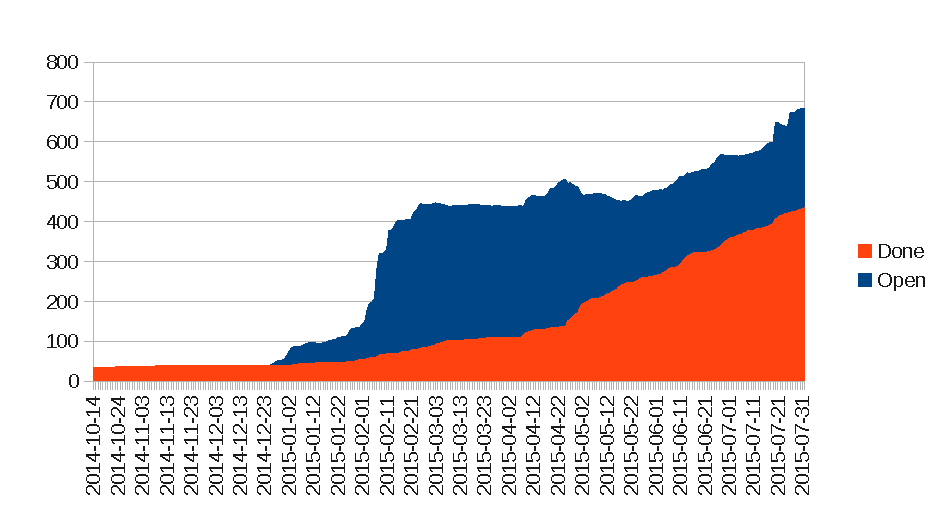
\includegraphics[width=\paperwidth]{images/bug_chart.pdf}
  };
 \end{tikzpicture}
\end{frame}

{
\usebackgroundtemplate{%
 \begin{tikzpicture}[remember picture,overlay]%
  \node[shift={(-0.15\paperwidth, 0.4\paperheight)},at=(current page.south east)] {
    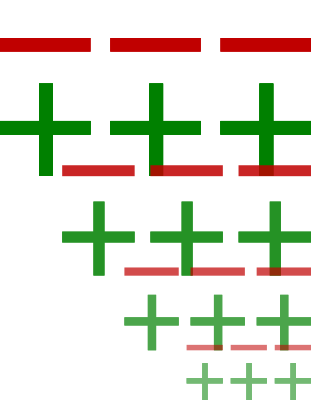
\includegraphics[width=0.2\paperwidth]{images/diffoscope_logo.png}
  };
 \end{tikzpicture}%
}
\begin{frame}{diffoscope}
 \frametitle{Depurando problemas: diffoscope}

 \begin{itemize}
  \item Examina las diferencias \textbf{en profundidad}
  \item Salidas de HTML o de texto plano que muestran las diferencias
  \item Desempaqueta recursivamente los archivos
  \item Busca la legibilidad humana:
   \begin{itemize}
    \item Descomprime PDF
    \item Desarma binarios
    \item Desempaqueta archivos Gettext
    \item … \textit{fácil de extender a nuevos formatos de archivo}
   \end{itemize}
  \item Retrocede a la comparación binaria
 \end{itemize}
 \vfill
 \begin{center}
  \url{http://diffoscope.org/}\\
  {\footnotesize \color{gray}{(formely known as \texttt{debbindiff})}}
 \end{center}
\end{frame}
}

\begin{frame}
 \frametitle{Ejemplo de diffoscope (salida de HTML)}

 \begin{center}
  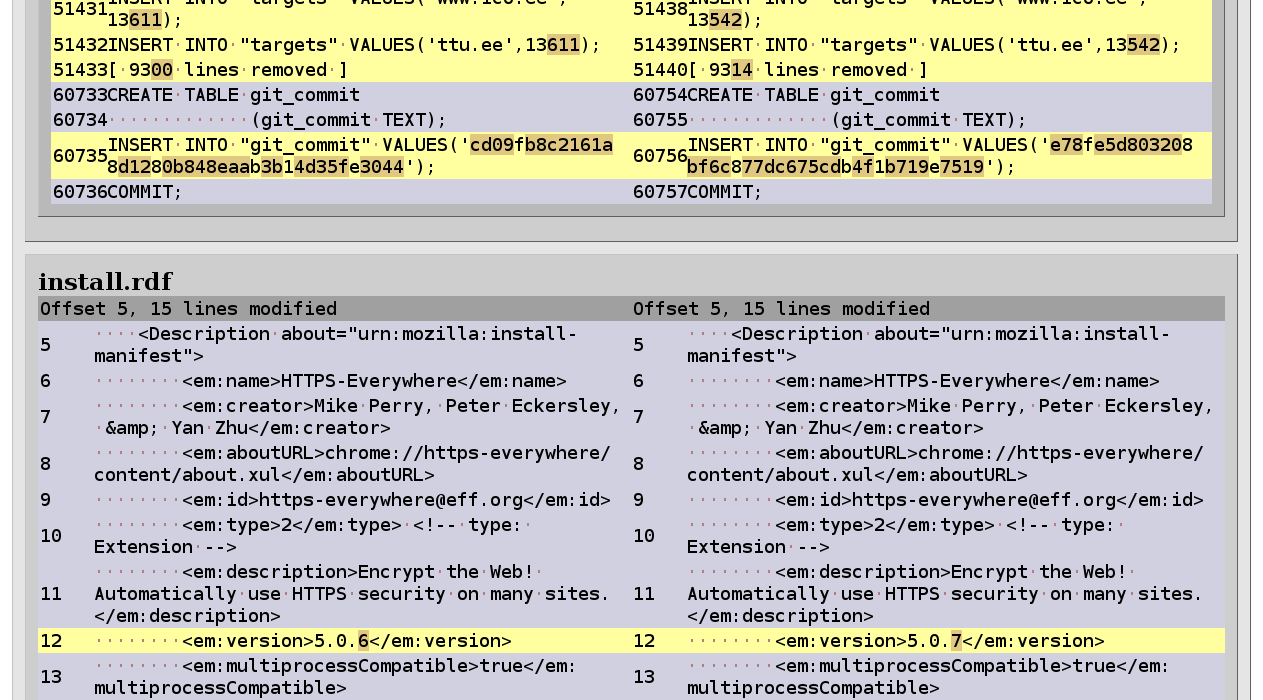
\includegraphics[width=0.9\paperwidth]{images/diffoscope_example_html.png}
 \end{center}
\end{frame}

\begin{frame}
 \frametitle{Ejemplo de diffoscope (salida de texto)}

 \begin{center}
  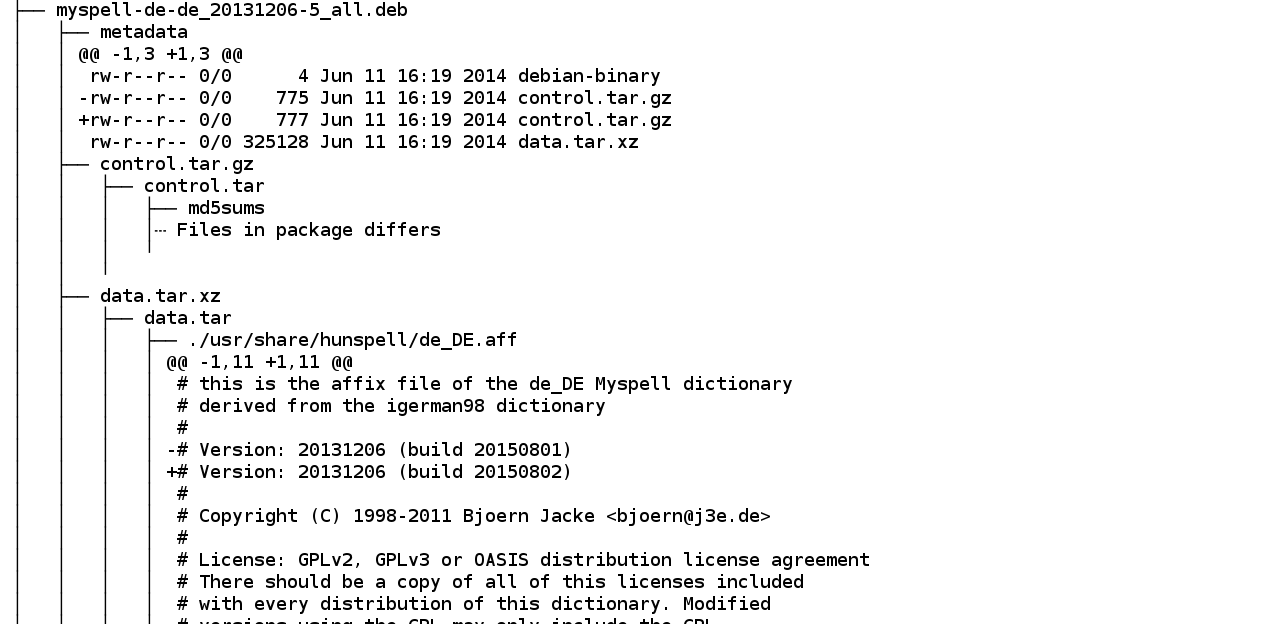
\includegraphics[width=0.9\paperwidth]{images/diffoscope_example_text.png}
 \end{center}
\end{frame}

\begin{frame}
 \frametitle{strip-nondeterminism}

 \begin{itemize}
  \item Normaliza varios formatos de archivo
  \item Actualmente maneja:
   \begin{itemize}
    \item archivos ar (\texttt{.a})
    \item gzip
    \item Java jar
    \item Javadoc HTML
    \item Maven \texttt{pom.properties}
    \item PNG
    \item archivos ZIP
    \item … \textit{extensible a nuevos formatos}
   \end{itemize}
  \item Escrito en Perl (como \texttt{dpkg-dev})
 \end{itemize}
 \vfill
 \begin{center}\small
  \url{git://git.debian.org/reproducible/strip-nondeterminism.git}
 \end{center}
\end{frame}

\begin{frame}
 \frametitle{Recursos}

 \begin{itemize}
  \item Reproducible Builds HOWTO \\
   \url{https://wiki.debian.org/ReproducibleBuilds/Howto}
  \item<2-> Wiki de Debian Reproducible Builds \\
   \url{https://wiki.debian.org/ReproducibleBuilds}
   \item<2-> Descripción general de estadísticas sobre construcciones reproducibles \\
   \url{https://tests.reproducible-builds.org/debian/reproducible.html}
  \item<3> Construcción doble diversa \\
   \url{http://www.dwheeler.com/trusting-trust/}
 \end{itemize}
\end{frame}

\section{Estado en Debian}

\begin{frame}
	\frametitle{Resumen de Debian - situación en Stretch (Debian 9)}
 \begin{itemize}
  \item Esto es/fue una prueba de concepto, Debian no es ni 94\% reproducible ni
  86\% (10\% > ¡2,500 paquetes fuente!).
  \item<2-4> ¡Todos nuestros cambios requeridos han sido incluidos en Stretch!
  \item<3-4> El 94\% de los paquetes fuente en Stretch pueden construir paquetes reproducibles.. Pero menos del 20\% de los binarios publicados son reproducibles...
  \item<3-4> Porque, Debian no (¿todavía?) hace reconstrucciones completas antes de
   liberar una nueva versión... así las cosas estarían en el archivo que no es reproducible a menos que sea
   reconstruido.
  \item<4> Y después entonces no distribuiríamos archivos \texttt{.buildinfo} todavía.
   Eso (y las herramientas de usuario) aún necesitan más \it{diseño} y código.
 \end{itemize}
\end{frame}

\begin{frame}
	\frametitle{Resumen de Debian - situación para derivadas y el futuro}
 \begin{itemize}
  \item El código fuente de Stretch es reproducible en un 94\% y todos los cambios requeridos están incluidos.
  \item Entonces otros, (por ejemplo Canonical) pueden tomar nuestro trabajo ahora y hacer Ubuntu 18.04
  (parcialmente) reproducible...
  \item<2-4> Debian 10 Buster, será parcialmente reproducible en 2019.
  \item<3-4> Desde agosto de 2017 \texttt{debian-policy} establece que los paquetes \textbf{deben} ser reproducibles.
  \item<4> Esperamos que \texttt{debian-policy} establezca 100\%
	  construcciones reproducibles («\textbf{deben de serlo}») para Debian 11 Bullseye en 2021. Y aún así, ahí pueden ser excepciones...
 \end{itemize}
\end{frame}

\section{¿Quieres ayudar?}

\begin{frame}
 \frametitle{Como desarrollador}
 \begin{itemize}
  \item Deja de usar las fechas de construcción
  \item Utiliza \texttt{SOURCE\_DATE\_EPOCH} en su lugar
  \item Visita \url{https://reproducible-builds.org/specs/}
 \end{itemize}
\end{frame}

\begin{frame}
 \frametitle{Participa aprendiendo haciendo}

 \begin{itemize}
  \item Prueba por ti mismo:
   \begin{itemize}
    \item Construye algo dos veces, ejecuta Diffoscope en los resultados
    \begin{itemize}
     \item Para obtener mejores resultados, usa nuestro repositorio "reproducible", \texttt{pbuilder} y una configuración personalizada
    \end{itemize}
   \end{itemize}
  \item Documentos en la web: \\
    \small{\url{https://reproducible-builds.org/docs/}} \\
    \small{\url{https://wiki.debian.org/ReproducibleBuilds/ExperimentalToolchain}}
  \item Pide ayuda en nuestros canales \texttt{\#debian-reproducible} y \texttt{\#reproducible-builds} ambos en la red OFTC de chat IRC o en nuestras listas de correo: \\
    \small{\url{reproducible-builds@lists.alioth.debian.org}} \\
    \small{\url{rb-general@lists.reproducible-builds.org}} 
 \end{itemize}
\end{frame}

\begin{frame}
 \frametitle{¡Únete al equipo!}

 \begin{itemize}
  \item ¿Por qué?
   \begin{itemize}
    \item Encantador grupo de personas
    \item Aprende algo nuevo cada día
    \item ¡Transforma el mundo (del software y más allá)!
   \end{itemize}
  \item ¿Qué hacemos?
   \begin{itemize}
    \item Revisar paquetes
    \item Identificar problemas y documentar soluciones
    \item \texttt{reproducible.d.n}, diffoscope, strip-nondeterminism
    \item Proponer cambios para las cadenas de herramientas (toolchain)
    \item Enviar parches para paquetes individuales
    \item Escribir más documentación general y correr la voz por el mundo
   \end{itemize}
 \end{itemize}
\end{frame}

\begin{frame}
 \frametitle{¡Únete al equipo!}

\begin{itemize}
    \item ¿Cómo empezar?
   \begin{itemize}
    \item Háblame aquí o habla con nosotros en IRC o por correo electrónico.
    \item Plática de Mike y Seth de 31c3 sobre motivaciones \url{https://media.ccc.de/v/31c3_-_6240_-_en_-_saal_g_-_201412271400_-_reproducible_builds_-_mike_perry_-_seth_schoen_-_hans_steiner}
    \item Plática de Lunar sobre la solución de problemas reproducibles en el CCCamp 15 \url{https://media.ccc.de/v/camp2015-6657-how_to_make_your_software_build_reproducibly}
    \item Hay mucha documentación
    \item Experimenta - aprende haciendo
   \end{itemize}
 \end{itemize}
\end{frame}

\section{¿Preguntas?}

\begin{frame}
 \frametitle{¿Preguntas, comentarios, ideas?}

 \begin{itemize}
  \item \url{https://reproducible-builds.org}
  \item \url{https://reproducible.debian.net}
  \item \texttt{\#debian-reproducible} en \texttt{irc.OFTC.net}
  \item \texttt{\#reproducible-builds} en \texttt{irc.OFTC.net}
 \end{itemize}
\end{frame}

\section{Créditos}

\begin{frame}
 \frametitle{Créditos}

 \begin{itemize}
  \item Contenido original «How to make your software build reproducibly» por Lunar
  \item Contenido original «Beyond reproducible builds» por Chris Lamb (lamby) y Holger ’h01ger’ Levsen
  \item Contenido original «Reproducible builds where do we want to be tomorrow» por Holger ’h01ger’ Levsen
  \item Traducción al español, edición y actualización por Jonathan Bustillos (Jathan)
 \end{itemize}
\end{frame}

\section{Referencias}

\begin{frame}
 \frametitle{Referencias}

 \begin{itemize}
  \item \url{https://wiki.debian.org/ReproducibleBuilds/About}
  \item \url{https://reproducible-builds.org/}
  \item \url{https://reproducible-builds.org/docs/definition/}
  \item \url{https://reproducible.alioth.debian.org/presentations/2015-08-13-CCCamp15.pdf}
  \item \url{https://events.ccc.de/congress/2014/Fahrplan/system/attachments/2491/original/2014CCCReproducible.pdf}
  \item \url{http://meetings-archive.debian.net/pub/debian-meetings/2015/mini-debconf-cambridge/slides/2015-11-08-Beyond-reproducible-builds.pdf}
  \item \url{https://anonscm.debian.org/cgit/reproducible/presentations.git/tree/2017-10-25-OSSE/}
  
 \end{itemize}
\end{frame}

\begin{frame}
 \frametitle{¡Gracias!}

 \begin{itemize}
  \item Equipo Debian Reproducible Builds \\
        {\small (¡Eres \textbf{tan} increíble!)}
  \item Linux Foundation y Core Infrastructure Initiative
\end{itemize}

 \begin{center}
  
\includegraphics[height=0.1\paperheight]{images/linux_foundation_logo.png}
  \hspace{0.1\paperwidth}
  
\includegraphics[height=0.1\paperheight]{images/cii_logo.png}
 \end{center}

 \vfill
 \begin{center}
  \resizebox{0.8\textwidth}{!}{%
   \begin{tabular}{rl}
    \texttt{jathanblackred@openmailbox.org} & \texttt{3006 B194 2622 24C7 1607} \\
                               & \texttt{F72B 52E4 5D29 AA34 EFC5} 
   \end{tabular}
  }
 \end{center}
\end{frame}

\begin{frame}
 \frametitle{¡Gracias!}

 \begin{center}
  
\includegraphics[height=0.5\paperheight]{images/CC-BY-NC-SA1.png}
 \end{center}

 \vfill
 \begin{center}
  \resizebox{0.8\textwidth}{!}{%
   \begin{tabular}{rl}
    \texttt{jathanblackred@openmailbox.org} & \texttt{3006 B194 2622 24C7 1607} \\
                               & \texttt{F72B 52E4 5D29 AA34 EFC5} 
   \end{tabular}
  }
 \end{center}
\end{frame}

\end{document}
